\labelsection{Results and Observations}{subsec:results_and_observations}
In the next sections we will investigate the questions we posed in the previous chapter.
After that, we will gather our findings to form an judgement of the validity of our hypothesis.

\todo{Observations + possible explanations}
\todo{How do the results relate to hypothesis?}
\todo{Error analysis}
\todo{Comparison between text n-grams and concept maps/co-occurrence graphs}
\todo{Look at concepts used in concept maps: frequency in whole corpus, ...}

\subquestionref{question:structure_diversity}
To investigate whether concept maps are useful for text classification, we first look at the structure of concept maps.
Our hypothesis especially highlights the structure of the concept maps since it is one of the main differences to other text representation.
Finding out whether the structure of concept maps is heterogeneous therefore is a first crucial step.

In Table \ref{table:graph_statistics}, we gathered metrics about the connectedness of concept maps and co-occurrence graphs with window size 1 for comparison.
One thing that immediately becomes apparent is the compression factor of the concept maps: on average, only approximately 8\% of the original text-content is retained in the concept maps.
This compression is useful for tasks like text summarization where only important concepts should be kept from the underlying text.

One consequence of the compression can be seen when looking at the connectedness of the concept maps.
On average, concept maps only have 1.36 edges per node. The minimum number of edges per node is 1 since we removed all unconnected nodes.
So, concept maps do not only have few nodes, because of the compression, but also a relatively low number of edges between them.
This is most likely due to the small length of the underlying texts.
The shortness of the text results in a lower number of occurrences of some concept in the text, ie. most of the concepts occur only once in a text.
To address this issue, we then searched for a dataset with longer texts per document.

\begin{table}[htb!]
	\centering
	\begin{tabular}{lcccccc}
		{} &  \multicolumn{2}{c}{\#nodes/\#words} &  \multicolumn{2}{c}{\#edges/\#nodes} & \multicolumn{2}{c}{\#nodes/graph} \\
		{} & concept map &  co-occurrence & concept map & co-occurrence & concept map & co-occurrence\\
		\midrule
		ling-spam       & 0.05 & 0.23 & 1.32 & 2.86 & 45.95 & 4.11 \\
		ng20            & 0.05 & 0.18 & 1.38 & 2.71 & 584.63 & 87.52 \\
		reuters-21578   & 0.09 & 0.21 & 1.46 & 2.86 & 63.07 & 13.20 \\
		review\_polarity & 0.08 & 0.20 & 1.42 & 2.67 & 50.36 & 10.55 \\
		rotten\_imdb     & 0.09 & 0.30 & 1.22 & 1.70 & 52.09 & 11.23 \\
		tagmynews       & 0.13 & 0.37 & 1.30 & 1.81 & 52.74 & 13.25 \\
		webkb           & 0.05 & 0.22 & 1.39 & 3.01 & 55.69 & 5.36 \\
		\midrule
		\O{}            & 0.08 & 0.24 & 1.36 & 2.52 & 129.22 & 20.75 \\
		\bottomrule
	\end{tabular}
	\caption[Statistics: Graphs]{Graph statistics. \textit{\#words} is the number of words in the whole text dataset. The metrics for co-occurrence graphs are obtained using a window size of 1. The \textit{\#nodes/\#words} metric corresponds to a compression factor. Note that, on average, the concept maps have a compression factor of 8\% compared to the 24\% of co-occurrence graphs. This means that co-occurrence graphs have approximately three times more node labels than concept maps. The \textit{\#edges/\#nodes} metric is an indicator for the connectedness of the graphs. Because we remove nodes which have no edge to other nodes, the \textit{\#edges/\#nodes} metric captures the average degree of the nodes. Looking at that metric we also see that, on average, the co-occurrence graphs with window size 1 have roughly twice as much edges per node as concept maps.}\label{table:graph_statistics}
\end{table}

\todo{New dataset! Statistics}
\todo{Add statistics about \# of occurrences of concepts in graphs}

Another hint for the un-connectedness of concept maps is the number of connected components.
In Table \ref{table:connected_component_percentage_per_size} we can see that most of the graphs have more than one connected component. Together with the observation of the low number of nodes per graph, this also implies the low connectedness of concept maps.
In this table we also report the percentage of connected components of size $\{2,3,4\}$ to the total number of connected components.
The results in this table show that the bulk of concept maps consist of small connected components and are generally quite un-connected. Connected components of size 2 and 3, ie. containing 2 or 3 nodes, make up 80 \% of all connected components.

In Figure \ref{fig:histogram_connected_components} we also plotted an histogram of the number of connected components per graph for \textit{ng20}.
In Figure \ref{fig:graph_examples} shows examples of concept maps and co-occurrence graphs with different window sizes.

\begin{table}[htb!]
\centering
\begin{tabular}{lrrrr}
	{} &  $|s_c|=2$ &  $|s_c|=3$ &  $|s_c|=4$ & $|s_{all}| > 1$ \\
	\midrule
	ling-spam       & 63.8 & 19.5 & 6.9 & 89.6 \\
	ng20            & 65.2 & 19.4 & 6.9 & 72.2 \\
	nyt\_200         & 61.4 & 19.8 & 7.7 & 100.0 \\
	r8              & 54.3 & 21.2 & 9.0 & 77.8 \\
	review\_polarity & 62.0 & 20.4 & 7.5 & 100.0 \\
	rotten\_imdb     & 66.9 & 23.6 & 6.9 & 19.1 \\
	tagmynews       & 54.2 & 28.3 & 11.2 & 31.7 \\
	ted\_talks       & 62.6 & 18.4 & 6.9 & 99.4 \\
	\midrule
	\O            & \% 61.3 & \% 21.3 & \% 7.9 & \% 73.7 \\
	\bottomrule
\end{tabular}
\caption[Statistics: Percentage of connected components size]{Percentage of connected component size of concept maps per dataset. $|s_c|=n$ corresponds to the size of the connected component and the percentage signifies how many connected component in the whole dataset have this size, eg. when $|s_c|=2$ has a 50\% share it means that 50\% of all connected components in all graphs have the size 2. $|s_{all}| > 1$ stands for the percentage of graphs that consist of more than one connected component, eg. when $|s_{all}| > 1$ is 50\% it means that 50\% of all graphs have more than one connected component.}\label{table:connected_component_percentage_per_size}
\end{table}

\begin{figure}[htb!]
\centering
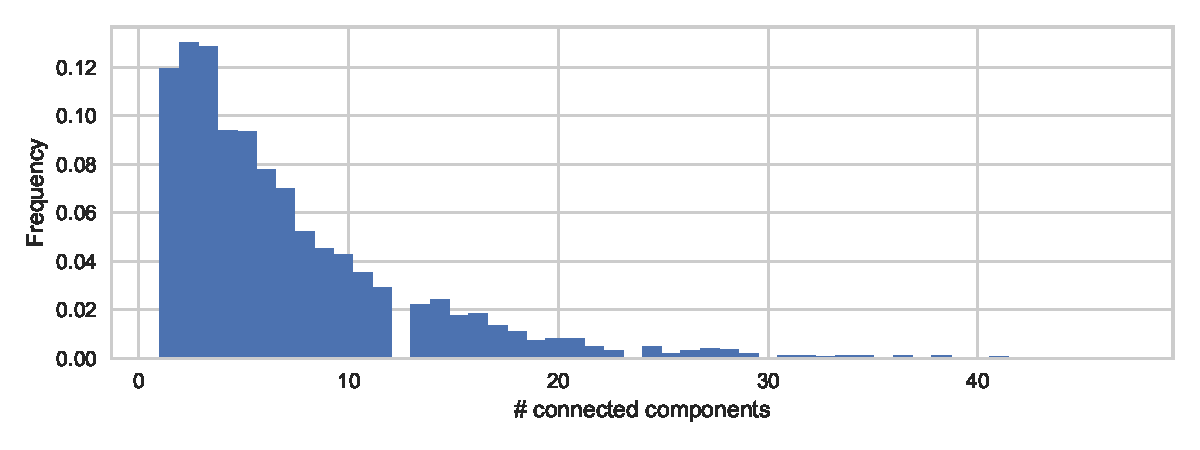
\includegraphics[width=0.8\linewidth]{assets/figures/hist-connected-components-ling-spam-CMap.pdf}
\caption[Statistics: Histogram of connected components per concept map]{Histogram of connected components per concept map. From the \textit{ling-spam} dataset.}\label{fig:histogram_connected_components}
\end{figure}

\begin{figure}[htb!]
	\centering
	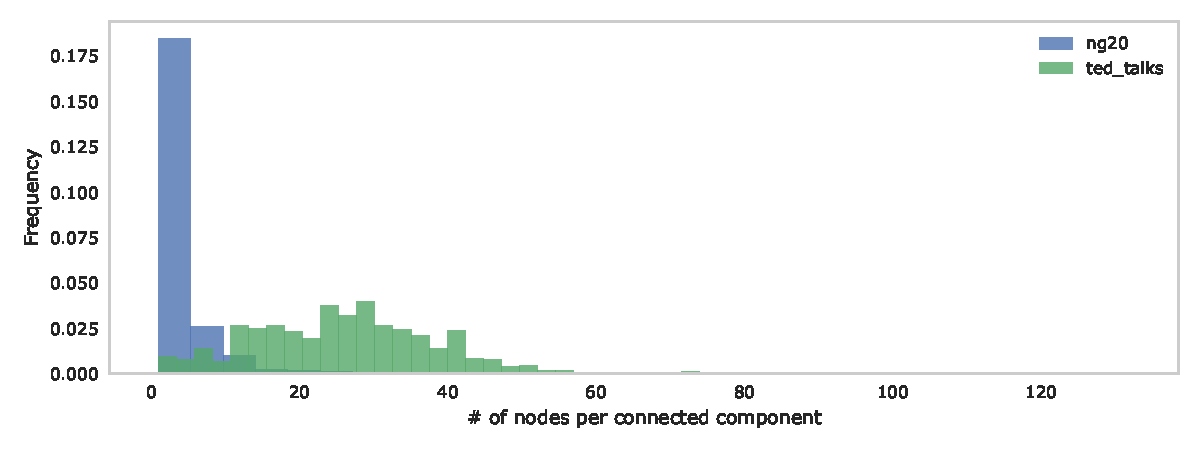
\includegraphics[width=0.9\linewidth]{assets/figures/connected_component_size_comparison.pdf}
	\caption[Statistics: Histogram of size of connectec components]{Histogram of the size of connected components, ie. the number of nodes per connected component, of concept maps for two datasets. The distribution of the size of connected components varies greatly between different datasets. In this instance, the \textit{ng20} dataset has mostly small connected components while the \textit{ted\_talks} dataset has bigger connected components. This is most likely due to the fact that the \textit{ted\_talks} dataset consists of longer, coherent texts while the \textit{ling-spam} texts are shorter as well as more informal.}
	\label{fig:histogram_connected_component_size}
\end{figure}

\begin{figure}[htb!]
\centering
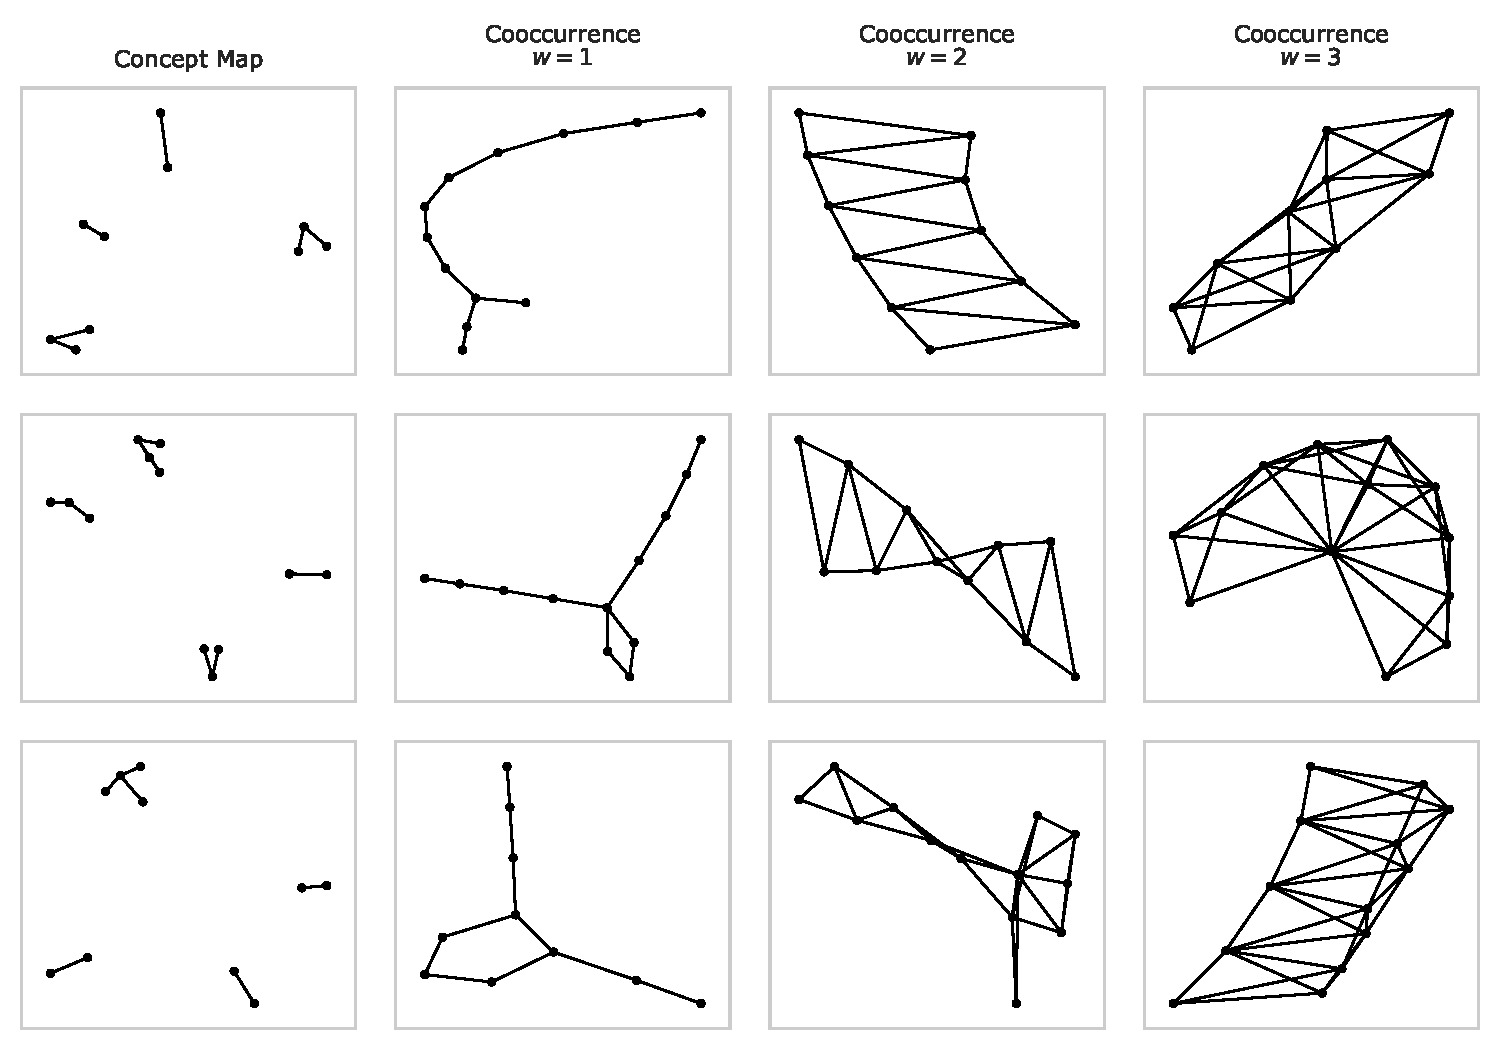
\includegraphics[width=0.7\linewidth]{assets/figures/examples_graphs.pdf}
\caption[Examples: Graph types]{Graph examples per type. Three random examples are shown per type. $w$ stands for the window size of the co-occurrence grpah. The concept map examples all have more than one connected component, while all co-occurrence graphs have only one. The shown graphs were randomly chosen from all graphs with $5 \leq |V| \leq 10$.Dataset: \textit{ng20}}\label{fig:graph_examples}
\end{figure}

\begin{figure}[htb!]
\centering
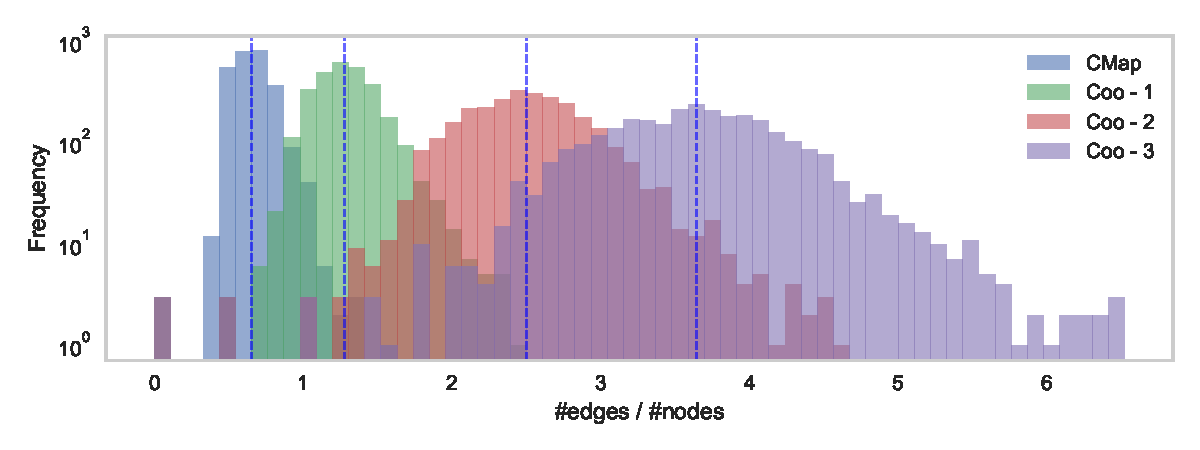
\includegraphics[width=0.7\linewidth]{assets/figures/hist-edgesnodes.pdf}
\caption[Statistics: Histogram of the number of edges divided by the number of nodes]{Histogram of the number of edges divided by the number of nodes. Per graph type. The lines correspond to the median value.}
\label{fig:histogram-edges-div-nodes-per-type}
\end{figure}

The co-occurrence graphs also have a simple structure.
Co-occurrence graphs are always connected, ie. the number of connected components is 1, or 0 in the case of an empty graph.
When the window size is 1, the graph is similar to a path, meaning that most of the nodes have a degree $< 2$. With increasing window size, the graph also gets more connected.

\begin{figure}[htb!]
	\centering
	{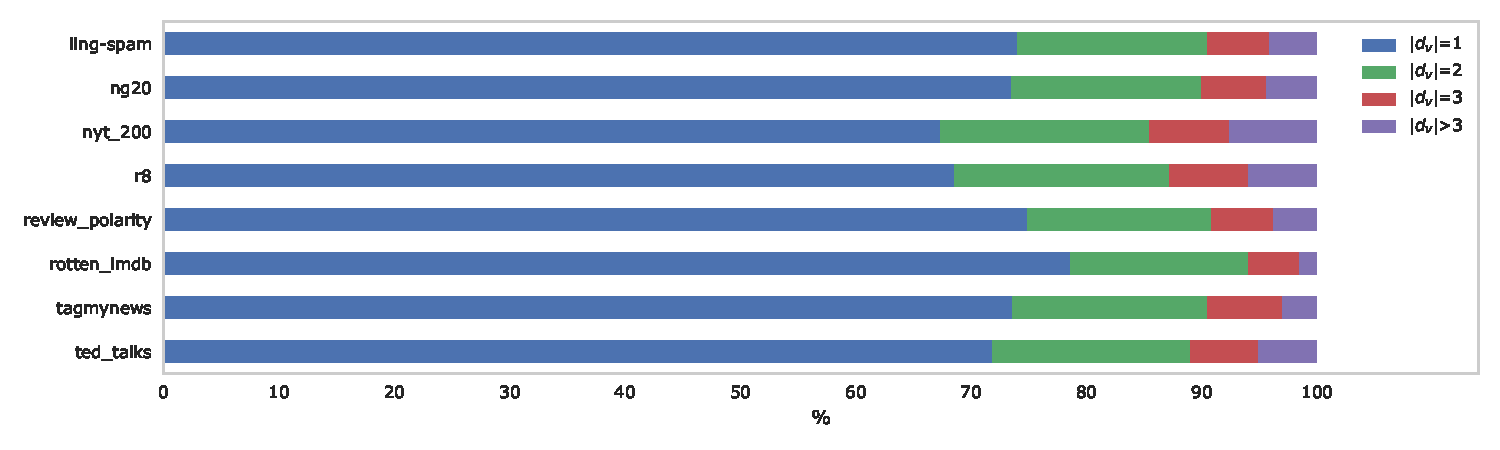
\includegraphics[width=\linewidth]{assets/figures/percentage_degree.pdf}%
		\caption[Statistics: Distribution of concept map node degrees]{%
			Distribution of concept map node degrees per datasets. $|d_v| = n$ stands for the percentage of nodes with degree $n$.
			We can see that well over 90\% of all nodes have a degree of $3$ or less.
		}%
		\label{fig:percentage_degree}}
\end{figure}

\subquestionref{question:importance_structure}
After investigating the structure of concept maps, we now aim to quantify the importance of the structure compared to the content.
The content, that is the node and edge labels, of concept maps are also captured in co-occurrence graphs and with conventional text-based approaches. So, the next interesting question about concept maps is, how much or whether the structure adds to the classification performance.
For this, we compare the results of using graph kernels which use \textbf{(a)} only the content, \textbf{(b)} only the structure and \textbf{(c)} both content and structure.

For \textbf{(a)} (content only), we use a kernel that discards all edges and uses only the labels of nodes and edges. Next, we create a bag-of-words vector representation out of the labels and edges.
In this step, we also evaluated using not only single words and counting them, but also using word n-grams of size 2, or bigrams.
For this, we create pairs of words by joining node labels together that have an edge between them.
The resulting vector representations of the graph then get fed into a conventional classifier, in our case a SVM.

For \textbf{(b)} (structure only), we use a modified version of the Weisfeiler-Lehman graph kernel. Before applying the actual WL kernel, we discard all node labels and give every node in all graphs the same label, effectively ridding the graphs of content. Next, we apply the WL graph kernel. This variant of WL only takes the structure of the graph into account.
After executing WL on the graphs, we obtain the feature maps which get subsequently get fed into a SVM also.

For \textbf{(c)} (structure and content combined), we use the Weisfeiler-Lehman that takes both structure and content into account.

In Table \ref{table:table_results_structure_vs_content} we report the results obtained from these experiments.

\begin{table}[htb!]
\centering
\begin{tabular}{llrrr}
          & & \multicolumn{3}{c}{f1 macro} \\
Dataset & Type & \textbf{(a)} content only & \textbf{(b)} structure only & \textbf{(c)} combined\\
\midrule
ling-spam & concept map &  0.933020 &  0.468187 &  0.741138 \\
          & cooccurrence &  0.959041 &  0.519897 &  0.794719 \\
\midrule
ng20 & concept map &  0.592340 &  0.035334 &  0.263055 \\
          & cooccurrence &  0.679036 &  0.049227 &  0.511980 \\
\midrule
reuters-21578 & concept map &  0.241263 &  0.005962 &  0.085752 \\
          & cooccurrence &  0.293941 &  0.012733 &  0.229710 \\
\midrule
webkb & concept map &  0.472472 &  0.162010 &  0.222296 \\
          & cooccurrence &  0.714741 &  0.170633 &  0.472485 \\
\bottomrule
\end{tabular}
\caption[Results: Linearized vs. WL]{Comparison of linearized graph with CountVectorizer and results of WL}\label{table:table_results_structure_vs_content}
\end{table}

\todo{Interpret results!}
\todo{Ratio between (a), (b) to (c). Why is combined less good?}
\todo{Why do we not use the zero-th iteration, ie. counting the plain labels?}

\subquestionref{question:comparison_coo}

\todo{Co-occurrence:"Text kernel" performs nearly as well as normal text}
\todo{Co-occurrence: only minor decrease (1\%) in performance when only using nouns}
\begin{table}[htb!]
\centering
\begin{tabular}{lrrr}
&  concept\_map &  cooccurrence &   ratio \\
\midrule
ling-spam       &  0.7165 &  0.9112 &  0.7863 \\
ng20            &  0.2904 &  0.3964 &  0.7325 \\
review\_polarity &  0.5615 &  0.6656 &  0.8436 \\
rotten\_imdb     &  0.5786 &  0.8070 &  0.7170 \\
webkb           &  0.2763 &  0.5082 &  0.5438 \\
\bottomrule
\end{tabular}
\caption[Results: Co-Occurrence vs. Concept Maps]{Comparison of co-occurrence results with concept maps}\label{table:comparison_results_cooccurrence}
\end{table}

\subquestionref{question:comparison_text}
As one can see in Figure \ref{fig:results_cmap_vs_text}, the text-only- outperform graph-only approaches by a high margin.
This is most likely due to the high compression factor of concept maps and co-occurrence graphs.

\begin{figure}[htb!]
\centering
\missingfigure[figcolor=white]{}
\caption[Results: Concept Maps vs. Text]{Comparison of concept maps with text}
\label{fig:results_cmap_vs_text}
\end{figure}

\subquestionref{question:multi_labels}
As we can see in Figure \ref{?}, most concept map node labels consist of more than one word. 


\subquestionref{question:edge_labels}
In concept maps, an edge label can be combined with the label of its source and target nodes to form a sentence.
To evaluate how important the edge labels are, we first look at the occurrences of edge labels, ie. how often a unique edge label occurs in the concept maps of a whole dataset.
In Table \ref{table:edge_label_occurrences} we see that, on average, 76\% of all unique edge labels occur only once per dataset. For comparison, the percentage of unique words which only occur once in a text, on average, is often well below 50\% for our datasets.

\begin{table}[htb!]
	\centering
	\begin{tabular}{lrr}
		dataset &  $ \%_{unique} $ & $ \%_{all}$  \\
		\midrule
		ling-spam       & 69 & 27 \\
		ng20            & 73 & 30 \\
		nyt\_middle      & 73 & 32 \\
		nyt\_small       & 78 & 43 \\
		review\_polarity & 80 & 39 \\
		rotten\_imdb     & 80 & 47 \\
		tagmynews       & 75 & 39 \\
		ted\_talks       & 80 & 39 \\
		\midrule
		\O           & 76 & 37 \\
		\bottomrule
	\end{tabular}
	\caption[Statistics: Percentage of concept map labels occurring once]{Percentage of concept map edge labels occurring only once in the whole dataset.
		$ \%_{unique} $ corresponds to the percentage of edge labels which only occur once to the number of unique labels in the whole dataset, eg. $ \%_{unique} = 50\% $ would mean that 50\% of all unique edge labels occur only once.
		$ \%_{all}$ stands for the percentage of edge labels which occur only once to all labels (with duplicates), eg. $ \%_{all} = 50\%$ would mean that 50\% of all edge labels occur only once in the dataset.}\label{table:edge_label_occurrences}
\end{table}

When examining the most occurring edge labels per dataset, most of these most-frequent edge labels consist of stopwords or non-descriptive words like ``is", ``has", ``are".
These most-frequent edge labels, together with the edge labels which occur only once, form the bulk of all edge labels.

As a test for the importance of edge labels, we evaluate \textbf{(a)} a graph kernel which uses the edge labels against \textbf{(b)} a graph kernel which does not use edge labels.
For both, \textbf{(a)} and \textbf{(b)}, we use a graph kernel which first converts the graphs into a set of labels and then counts the number of these labels for each graph.
For \textbf{(a)} we use the edge labels, for \textbf{(b)} we omit them.

\begin{table}[htb!]
	\centering
\begin{tabular}{lrr}
	{} & \multicolumn{2}{c}{edge labels} \\
	dataset & without & with \\
	\midrule
	ling-spam  & 0.926 & \textbf{0.932} \\
	ng20       & \textbf{0.595} & 0.592 \\
	nyt\_middle & \textbf{0.795} & 0.793 \\
	nyt\_small  & 0.720 &\textbf{ 0.740} \\
	ted\_talks  & \textbf{0.455} & 0.418 \\
	\bottomrule
\end{tabular}
\caption[Results: Graph Kernel with and without edge labels]{Classification results for a graph kernel either using or omitting edge labels.}\label{table:edge_label_classification}
\end{table}

As we can see in Table \ref{table:edge_label_classification}, omitting or using the edge labels result in comparable performance.
For some datasets, omitting the edge label actually improves the classification score.

\todo{These facts all indicate that edge labels, while crucial and useful for text-summarization and the subsequent use by a human, seem to have limited use in graph classification.}

\subquestionref{question:infrequent_nodelabels}
In Figure \ref{fig:percentage_distribution_concept_occurrences} we can see that, depending on the dataset, between 75\% to 90\% of all node labels occur only once per dataset.
This is also common in texts where most words also only occur once per dataset.
 
\begin{figure}[htb!]
	\centering{\includegraphics[width=\linewidth]{assets/figures/tmp/percentage_distribution_concept_occurrences.pdf}}
	\caption[Statistics: Distribution concept occurrence]{Concept map node label occurrences per dataset. $|n_v| = i$ stands for the percentage of labels with $i$ occurrences in the dataset, eg. when $|n_v| = 1$ has 50\%, it would mean that 50\% of all unique concepts only occur once per dataset.}\label{fig:percentage_distribution_concept_occurrences}
\end{figure}

While in text-based approaches, infrequent words are either ignored or filtered out to reduce the vocabulary and subsequently the dimension of the feature vector, the infrequent node labels might pose a far greater problem for our approach.
As noted before, in our work, we capitalize on the Weisfeiler-Lehman graph kernel to extract useful features for subsequent classification.
In the context of WL, infrequent node labels might become a problem since a match becomes less likely with less occurring words, or a match even becomes impossible as in the case of node labels which occur only once.
When simply creating a feature vector by counting the node labels in each graph, infrequent node labels would not pose a problem.
WL on the other hand relies on exact matches of neighborhoods.
Thus, a node label which only occurs once would ``taint" its neighborhood, effectively making matches in its neighborhoods impossible.

\subquestionref{question:directed_vs_undirected}
The concept maps we extracted have directed edges.
In this question, we evaluate the usefulness of these two cases.
We compare the classification performance of using the directed versus un-directed case with the Weisfeiler-Lehman graph kernel.

When using WL with undirected edges, the neighbors $n_v$ of a node $v$ are all nodes $v'$ that are connected by an edge to $v$, or $n_v = \{v' | (v, v') \in E \lor (v', v ) \in E \}$.
With directed edges, on the other hand, the neighbors $n_v$ of a node $v$ are only nodes $v'$ where there exists a directed edge from $v$ to $v'$, or $n_v = \{v' | (v, v') \in E \}$.
So, the size of neighborhoods per node are expected to decrease, since there is an additional constraint to what constitutes a neighbor.

In Table \ref{table:results_directed_vs_undirected} we see the results of using WL with directed and un-directed edges.
In all datasets, apart from the \textit{ng20} dataset, the directed edges outperform the un-directed approach.

\begin{table}[htb!]
	\centering
\begin{tabular}{lrrr}
	dataset &  un-directed & directed &  difference \\
	\midrule
	ling-spam       &  0.6793 &  \textbf{0.7661} &  0.0867 \\
	ng20            &  \textbf{0.3923} &  0.3728 & -0.0195 \\
	nyt\_80          &  0.5713 &  \textbf{0.6489} &  0.0776 \\
	r8              &  0.4240 &  \textbf{0.5445} &  0.1206 \\
	review\_polarity &  0.5135 & \textbf{ 0.5736 }&  0.0601 \\
	rotten\_imdb     &  0.5274 &  \textbf{0.5484} &  0.0210 \\
	tagmynews       &  0.3426 &  \textbf{0.3803} &  0.0377 \\
	ted\_talks       &  0.1399 &  \textbf{0.1790} &  0.0391 \\
	\bottomrule
\end{tabular}
\caption[Results: WL with directed and un-directed edges]{Classification results when using directed versus un-directed edges with WL.}\label{table:results_directed_vs_undirected}
\end{table}

This is most likely due to the aforementioned property that the neighborhoods are smaller with directed edges, making exact matches of neighborhoods more probable.
Note that using directed edges in WL could be compared with using n-grams: when the order of words/nodes is fixed in one direction, vertices with no outgoing edges do not have a neighborhood. Thus they are, for all WL iterations, considered to be the same label, ie. they get no new color assigned.
Later on, we will also evaluate whether or how using (un-) directed edges affects the score when combining graph and text features.

\subquestionref{question:concept_map_size}
In most datasets, longer texts often result in higher classification performance.
So, an interesting question is whether the size of a concept map also correlates with its classification performance, ie. whether ``bigger" graphs in terms of the number of nodes and edges are easier to classify.
To test this, we classify the graphs with our standard approach, using the Weisfeiler-Lehman graph kernel, then a SVM to classify the feature maps.
In the next step, we look at the results for different graph sizes, binning them with quantiles, in our case 10 quantiles, or deciles.

\begin{figure}[htb!]
	\begin{subfigure}[t]{.5\linewidth}	{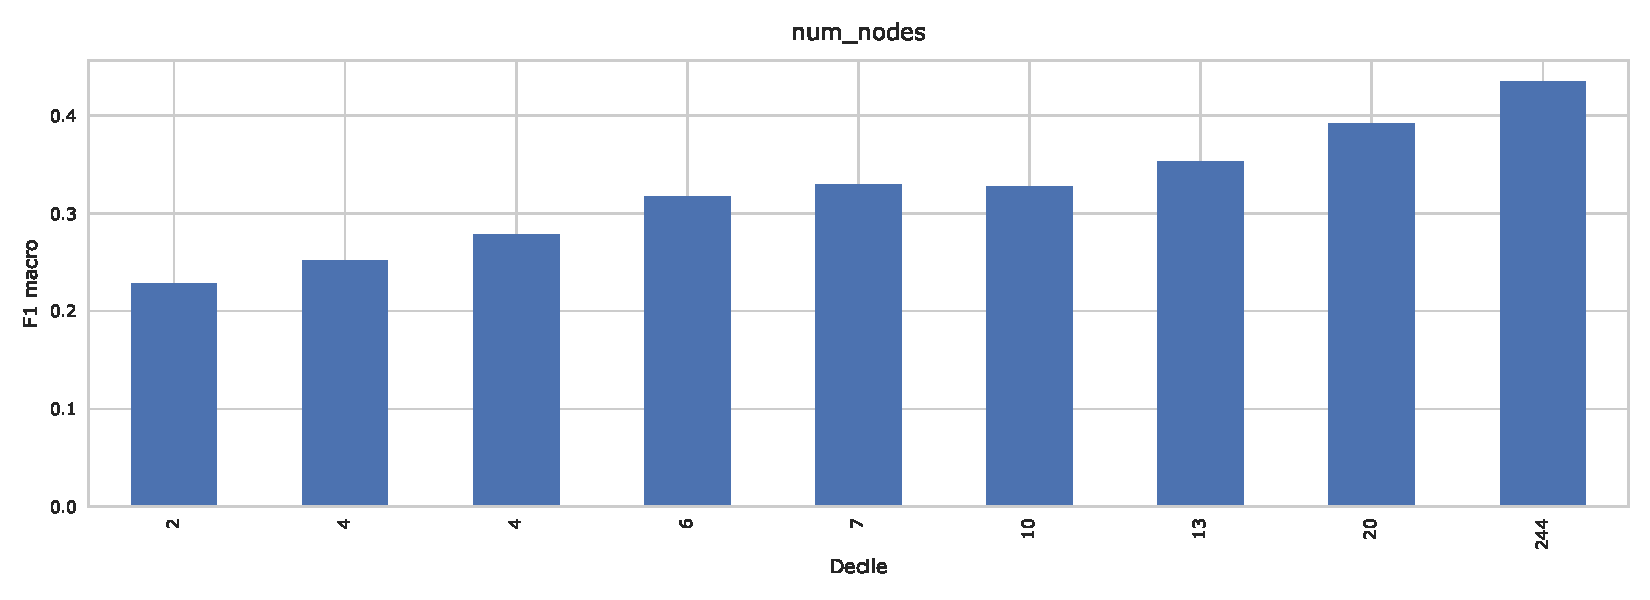
\includegraphics[width=\linewidth]{assets/figures/graph_binning_num_nodes.pdf}\label{fig:todo_1}}
	\caption{Graphs}
	\end{subfigure}
	\hfill
		\begin{subfigure}[t]{.5\linewidth}
	{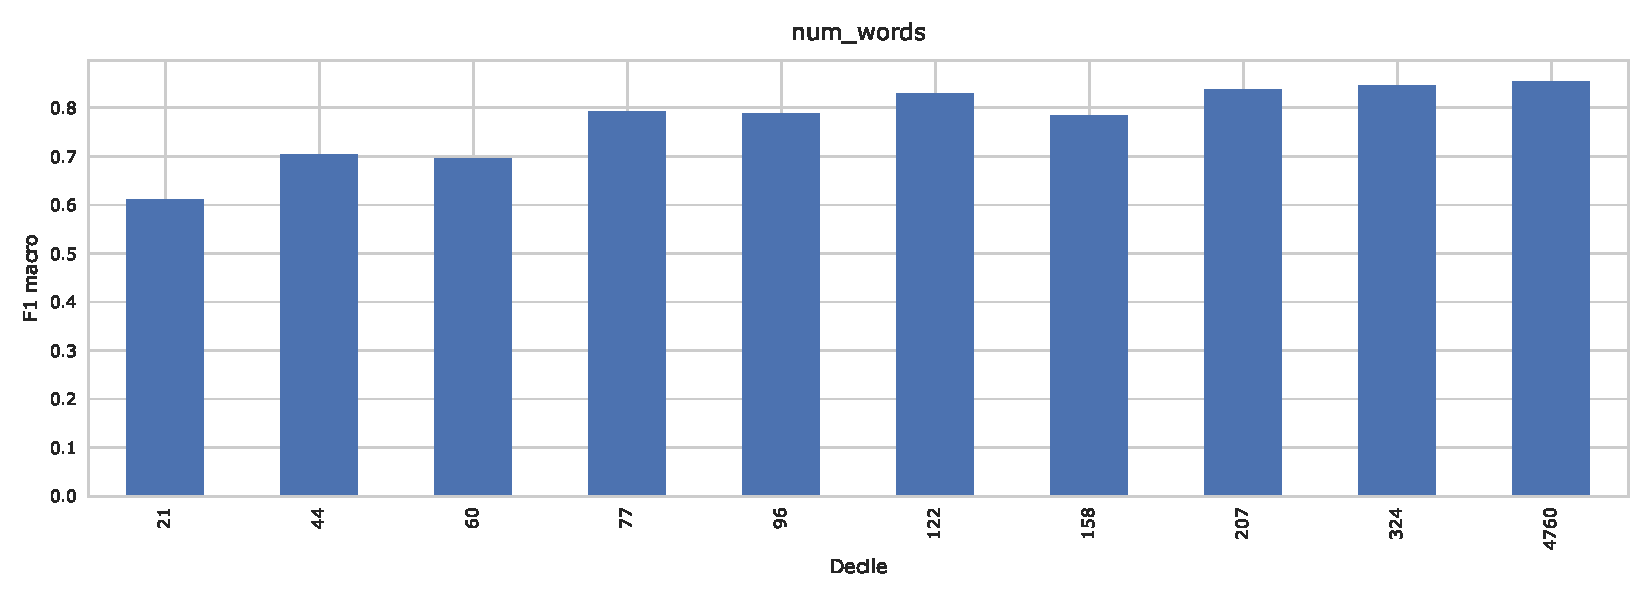
\includegraphics[width=\linewidth]{assets/figures/text_binning_num_words.pdf}\label{fig:todo_2}}
	\caption{Text}
	\end{subfigure}
	\caption[Statistics: Histogram of classification performance per graph/text size]{Classification performance per graph/text size. The x-axis corresponds to the size of the graph/text, the y-axis for the classification performance for graphs/text of that size. Dataset: \textit{ng20}}\label{fig:graph_size_performance}
\end{figure}

In Figure \ref{fig:graph_size_performance} we see an example for the \textit{ng20} dataset where we binned the different graph and text sizes and report the classification scores of documents with these sizes.
For this dataset, the results indicate that classification performance indeed correlates with the number of nodes of the concept map.
In other datasets, this correlation is not as distinguished.
\todo{Results for other datasets have to be inserted!}

\subquestionref{question:dataset_diversity}
\todo{?}

\subquestionref{question:comparison_combined}
As we have seen in the results of the last section, text-based approaches outperform graph-only approaches.
In this section we investigate how and whether the graph-based approaches improve the classification score when combined with text-based approaches.

For the text features we vectorized the text with a bag-of-words approach. We also tried features with tfidf.
For the graph features we used the Weisfeiler-Lehman algorithm since it is able to create feature map $\phi(G)$ for the graphs.
These feature maps can easily be concatenated with the text features.
For other graph kernels where an explicit feature map $\phi(G)$ can not be calculated, in order to combine graph- and text features, we would have needed to create a combined kernel that takes both text- and graph features into account and calculate a gram matrix.
The interpretability of this approach would be far lower since both graph- and text-features would be merged together in a single number without being able to distinguish the relative importance of the text- and graph features after creating the gram matrix.
In Table \ref{table:results_comparison_combined} we see the classification scores for the combined features for both co-occurrence graphs and concept maps.

As we see, the performance of the combined approached compared the text-only approach is comparable.
With some datasets, the combined approach is slightly better than the text-only approach. Especially for the ng20 dataset, we see an improvement of ca. 3\% over the text-only approach.
To test whether this difference in performance is due to chance, we used the permutation test
\todo{Add permutation test result}

To better understand the performance when combining text- and graph features, we also train a one-layer neural network, ie. a \textit{Perceptron}, with the combined features. After training we investigate the weights.
The weights, or coefficients, for each input feature are an indicator for the importance of that input feature.
Thus we can look at weights for the text features and compare them to weights for graph features.
This gives us an insight into the relative importance of text- and graph features.
In Figure \ref{fig:coefs_example_one_layer} we show an example of an one-layer neural net.
For our purposes, we do not look at single features, or input neurons, but on a range of features, namely the text and graph feature ranges since, in our case, the text- and graph features are concatenated.

\begin{figure}[htb!]
	\centering
	{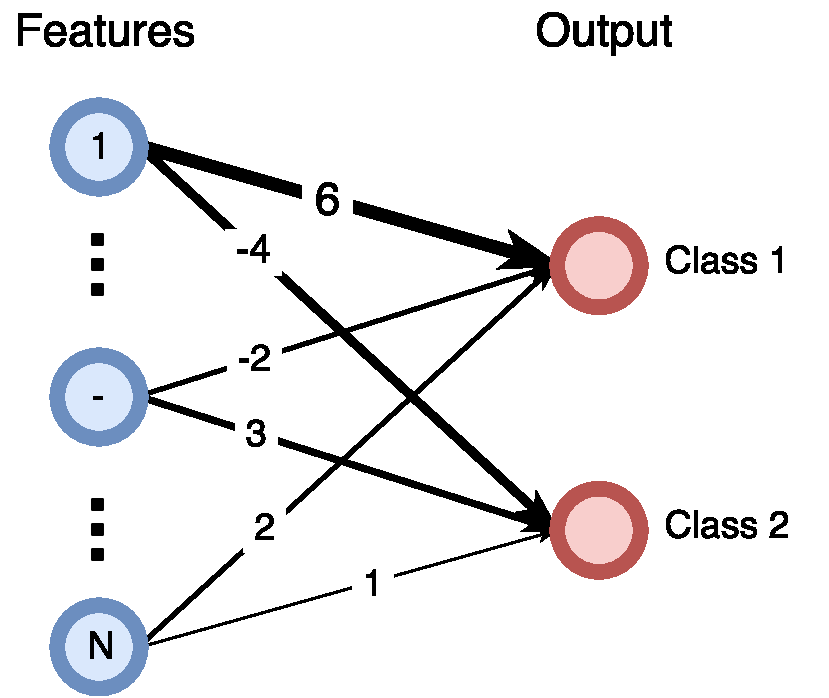
\includegraphics[width=0.5\linewidth]{assets/figures/coefs_example.pdf}%
		\caption[Example: One-layer neural net]{%
			Example of an one-layer neural net. The numbers on the line from input features to the output are weights.
			We examine these weights for single features to gain an insight into the importance the neural net assigned to a given feature. Since a feature contributes to all output neurons, we look at the sum of its absolute weights. Eg. for \textit{Feature 1} the sum of the absolute weights would be $|6| + |-4| = 10$ and for \textit{Feature n} it is $|2| + |1| = 3$, which gives us the hint that \textit{Feature 1} might be more important for the classification result than \textit{Feature N}.
			This analysis presupposes that the feature magnitudes, ie. the values of features, are normalized or - roughly speaking - in the same range on average, eg. \textit{Feature 1} does not take values between $[100, 200]$ while \textit{Feature N} takes values from $[0, 1]$, instead both feature values are roughly in the same range.
		}%
		\label{fig:coefs_example_one_layer}}
\end{figure}

Figure \ref{fig:combined_coefs_l1_l2_regularization} then shows an example of a weight analysis for the \textit{ng20} dataset and for two regularizations, namely \textit{L1} and \textit{L2}.

Both regularization terms are used to discourage ``big" weights, effectively forcing the training algorithm to chose important features to generalize the data instead of over-fitting the data.
While both \textit{L1} and \textit{L2} regularization discourage big weights, \textit{L1} penalizes small weights harder than \textit{L2}, leading to sparser models.
Therefore, the selection of important features is enforced more with \textit{L1} regularization.
We leverage this phenomenon to analyze how important the features, graph and text, are for classification.
When looking at the absolute sum of the weights of the trained one-layer neural net, we discover that using \textit{L1} regularization results in the text features becoming more important than graph features for classification.
While the difference of absolute sums of the coefficients does not seem especially high, it has to be noted that graph features are approximately only half as dense as text features.
Thus the contribution by graph features to the end result is even lower than the neural net coefficients indicate.

\begin{figure}[htb!]
	\centering
	{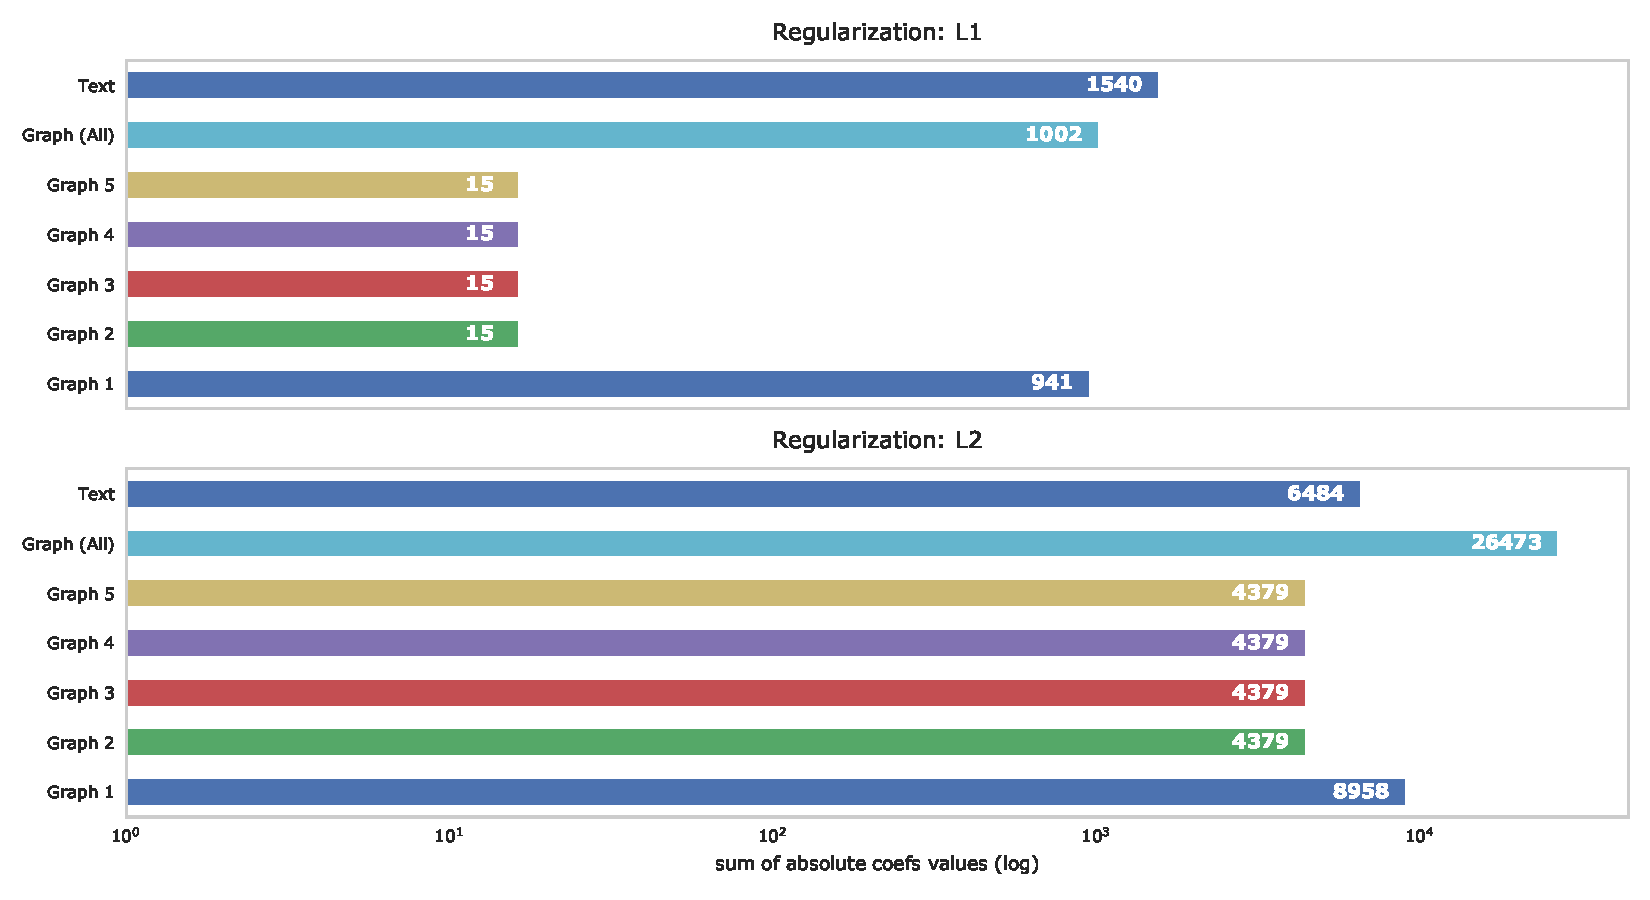
\includegraphics[width=\linewidth]{assets/figures/combined_coefs_l1_l2_regularization.pdf}%
		\caption[Statistics: Histogram of the trained weights of a one-layer neural net]{%
			Histogram of the trained one-layer neural net weights. The neural net was trained on the concatenated graph- and text features.
			Higher values indicate higher importance.
			\textit{Graph (All)} stands for the sum of all graph feature weights, while the \textit{Graph $N$} stand for the individual Weisfeiler-Lehman iterations.
			Higher iterations of WL take a bigger neighborhood into account.
			Dataset: \textit{ng20}.
		}%
		\label{fig:combined_coefs_l1_l2_regularization}}
\end{figure}

Another interesting result of this weight analysis is the importance the neural net assigns to the different Weisfeiler-Lehman iterations. In our example, we chose $h = 5$ as our WL iterations. The higher the iteration, the bigger the neighborhood that is considered by WL.
When looking at the importance of the first iteration and \textit{L1} regularization, \textit{Graph 1} in Figure \ref{fig:combined_coefs_l1_l2_regularization}, we see that while the neural net nearly discourages all higher WL iterations by assigning low weights, it assigns higher importance to the first iteration of WL, $941$ versus $15$.
The first iteration of WL takes only the immediate neighborhood into account, therefore matches are far more probable than matches in higher iterations.
In our example in Figure \ref{fig:combined_coefs_l1_l2_regularization}, \textit{L1}- outperformed \textit{L2} regularization by a high margin, approximately 7\% difference in the \textit{F1} macro score.
Yet it has to be noted that no hyper-parameter tuning was performed and only a simple train-/test split was used.

\todo{Cite where it is said that l1 regularization produces sparse features}


\begin{table}[htb!]
\centering
\begin{tabular}{llcc}
  &  & \multicolumn{2}{c}{Graph type} \\
   dataset   & &  Concept Map &  Co-Occurrence \\
\midrule
ling-spam 
          & graph only &  0.741138 &  0.794719\\
          & combined &  0.986928 &  0.977104\\
          & text only & \multicolumn{2}{c}{ 0.966179 }\\
\midrule
ng20 
          & graph only &  0.263055 &  0.511980\\
          & combined &  0.738239 &  0.690968\\
          & text only & \multicolumn{2}{c}{ 0.681245 }\\
\midrule
reuters-21578 
          & graph only &  0.085752 &  0.229710\\
          & combined &  0.264947 &  0.291086\\
          & text only & \multicolumn{2}{c}{ 0.320838 }\\
\midrule
webkb 
          & graph only &  0.222296 &  0.472485\\
          & combined &  0.722667 &  0.741964\\
          & text only & \multicolumn{2}{c}{ 0.702095 }\\	
\bottomrule
\end{tabular}
\caption[Results: Combined text- and graph features]{Comparison of classification using both concept maps and text. TODO: Add standard deviations}%
\label{table:results_comparison_combined}
\end{table}

\subquestionref{question:comparison_runtime}
\todo{?}

\labelsection{Related And Intermediate Observations}{subsec:related_and_intermediate_observation}
In this section we report observations which are not directly related to our questions or hypothesis, yet they nevertheless have provided us more insights into our analysis.

\subsection{Weisfeiler-Lehman $\phi$ Feature Map Visualization}
When debugging our Weisfeiler-Lehman implementation and extensions, we often wanted to see the effect on the feature vectors created by WL.
For this, we plotted the feature vector $\phi(G)$ for each graph $G$ for several WL iterations.
In Figure \ref{fig:phi_distribution_example} we see an example of such a $\phi$ distribution plot.

\begin{figure}[htb!]
	\centering
	{\includegraphics{assets/figures/wl_phi_distributions/dataset_graph_concept_map_ng20-v3_phi_npy.png}
		\caption[Example: $\phi$ distribution plot]{%
			Example of a WL $\phi$ distribution plot.
			For each WL iteration $h$, the horizontal $x$-axis corresponds to the concept maps in the datasets, while the vertical $y$-axis corresponds to the indices of $\phi(G)$ which are non-zero, ie. when there is a point at $x=0$ and $y=10$, the graph $G_0$ has the label $10$.
			There are as many points in this plot as there are vertices in the dataset.
			The colors of a point corresponds to the class of the graph, in this case the 20 classes of \textit{ng20}.
			The red line marks the number of vertices in the datasets which is also the dimension of the feature map $\phi$.
			Dataset: \textit{ng20}.
			\textit{Note: embedding this plot in a vector format  was not possible due to the sheer number of points to be drawn. The rasterized image seen here interpolates the individual points.}
		}%
		\label{fig:phi_distribution_example}}
\end{figure}

It has to be noted that we implemented WL where the labels are assigned when they are first encountered. That means that when we create the feature map $\phi(G_i)$ for graph $G_i$, we relabel the graph by assigning it a new multi-label by taking the neighborhood into account (\textit{recoloring}). In the next step, we compress the new multi-label by assigning it a new number if it has not been encountered before and save it in a multi-label-lookup. If the multi-label has been encountered before, ie. the multi-label is in the multi-label-lookup, we assign it the number it has been assigned before.
This is the \textit{label compression} step.
So, we iterate over the graphs one by one and create feature maps $\phi$.
When the first processed graph, $G_1$, has the new compressed labels $\{1, 2, \ldots, n\}$, the next processed graph, $G_2$, will have labels that are either \textbf{(1)} new, in which case they get a new, compressed label that is higher than $n$ or \textbf{(2)} they were already encountered in $G_1$, so they get the label from the lookup.
This way we get incrementing labels for each graph.
When we also sort the graphs by their assigned class, ie. all graphs of class $y_i$ are processed after another, then one can look at the labels that are assigned to each class and also see the nice pattern which arises in Figure \ref{fig:phi_distribution_example}.

This plot also gives an insight about the convergence of WL.
The highest encountered $\phi$ index in iteration $h=1$ must be higher or equal than the highest $\phi$ index encountered in $h=0$.
This is directly due to the fact that more colors are needed to color the graph nodes in higher iterations - if WL has not converged.
The number of labels, or colors, $|L_i|$ assigned in iteration $h=i$ must be smaller or equal than the labels for iteration $h=i+1$, ie. $|L_i| \leq |L_{i + 1}|$.
When $|L_i| = |L_{i + 1}|$, WL is said to have converged, ie. the number of colors will not change anymore.

In this figure, there is also a highest horizontal, green line.
This line signifies the highest $\phi$ index where there was a non-zero entry.
It also serves as a marker of the last compressed label number which was assigned in this dataset.

While this kind of plot is useful for analyzing the whole datasets at once, it becomes especially interesting when splitting the dataset into sets, eg. by splitting it into a stratified train- and test set.
When creating the feature maps $\phi$ for the graphs in the train set, for each WL iteration $h$ we save the multi-label-lookup which we can then use to create the feature maps for the test set.
The multi-label lookup therefor acts as a kind of continuation, saving the state of the WL iteration with all encountered labels.
Then, when creating the feature maps for the test set, we use the multi-label lookups to generate the feature maps in the same way, now for the graphs in the test set.
When plotting the train- and test set feature maps separated we can get interesting insights into the dataset and the concept maps.
For an example, see Figure \ref{fig:phi_distribution_train_test}.

\begin{figure}[htb!]
	\begin{subfigure}[t]{.49\linewidth}%
		{\includegraphics{assets/figures/wl_phi_distributions/dataset_graph_concept_map_ng20-v3_splitted_phi_npy_train.png}}\caption{Train}%
	\end{subfigure}%
	\begin{subfigure}[t]{.49\linewidth}%
		{\includegraphics{assets/figures/wl_phi_distributions/dataset_graph_concept_map_ng20-v3_splitted_phi_npy_test.png}}\caption{Test}%
	\end{subfigure}%
	\caption[Diagram: $\phi$ distribution plot for \textit{ng20}.]{WL $\phi$ distribution with a stratified train/test split.}%
	\label{fig:phi_distribution_train_test}
\end{figure}

While the train set looks nearly the same as if plotting the simple dataset without the split, the test set differs quite a bit.
Notice how, in the test set, there are ``clusters" around some regions for each of the classes. 
Keep in mind that the $y$-position of the point signifies the index $i$ in $\phi(G)$ for that graph.
Because of the aforementioned implementation, we now are able to see a pattern for each of the classes, namely the clusters.
For the test set, we can also see how many new labels have been found in a given iteration.
As we said before, the horizontal green line, in both plots, signifies the last label that has been encountered.
In the case of the split sets, it also marks the last label that has been encountered in the train set.

\todo{Usefulness of WL to get feeling for graph connectedness, uniqueness of structure, uniqueness of labels}

\subsection{Weisfeiler-Lehman extension}
With increasing iterations $h$ of the Weisfeiler-Lehman algorithm, exact matches of subtrees of height $h$ become more improbable.
In iteration 0, the Weisfeiler-Lehman only counts the number of node labels in the graphs, for iteration 1 it takes the immediate neighborhood of the nodes into account, for iteration 2 is takes the neighborhood of the neighborhood into account and so on.
So, \textbf{(1)} with higher iterations, the probability of having an exact match decreases.

Another difficulty arises for nodes with a high number of neighbors. \textbf{(2)} The probability of an exact match also decreases with a higher degree.

These two difficulties, \textbf{(1)} the increased difficulty of a match with higher iterations and \textbf{(2)} the increased difficulty of a match for nodes with higher degrees, are not addressed when using Weisfeiler-Lehman in its plain version. Both difficulties are neither encoded in the features maps nor are they considered when creating the gram matrix.

As a possible solution for these difficulties, we propose an extension to the plain Weisfeiler-Lehman algorithm.
Our extension augments the WL algorithm by adding node weights.
For each of the nodes in all graphs, we first calculate node weights which encode the importance of the nodes or the difficulty of getting an exact match in WL.
An example of such node weights are the node degree or node weights extracted with PageRank.
The node degree is an interesting metric for node weights since it actually encodes the size of the immediate neighborhood of a node and therefore could possibly address both problem \textbf{(1)} and \textbf{(2)}.

\todo{Explain how to actually use the node weights.}
\todo{Remark that the node weights could be seen as an additional metric of frequency: nodes with a higher degree have been in the text more frequently.}

Our other extension to the WL algorithm addresses problem \textbf{(1)}, the difficulty of having a match when the iteration increases.
To solve this difficulty, we propose weighting the features of each iteration.
The feature maps of WL consist of the concatenated feature maps for each iteration.
For this extension, we propose weighting the feature maps of each iteration $h$ by a factor given by a function $f(h)$.
So, for a feature map, $\phi(G)$, of a graph $G$ for $h=2$ iterations, the feature map can be decomposed into the feature maps of each of the two $h$ iterations:
\begin{equation*}
\phi(G)=(\phi_{h=1}(G), \phi_{h=2}(G))
\end{equation*}
We now propose to weight the individual feature maps by the factor determined by function $f(h)$, so:
\begin{equation*}
\phi_{f}(G)=(f(1) \cdot \phi_{h=1}(G), f(2) \cdot \phi_{h=2}(G))
\end{equation*}
So, basically the function $f(h)$ works as a decaying factor to decreasing iterations $h$.
When the function $f(h)$ increasing (steigend?), the increasing importance with higher iterations is encoded into the resulting feature map $\phi_f(G)$.

\todo{This is NOT a solution when feature-scaling is done.}